\documentclass[paper=a4,fontsize=10pt,dvipdfmx]{jlreq}
\usepackage[top=20truemm,bottom=20truemm,left=15truemm,right=15truemm]{geometry} %余白設定
\usepackage{amsmath,array} %数学に必要なパッケージ
\usepackage{tikz} %グラフ描画に必要なパッケージ
\usepackage{TeachersGuide}
\begin{document}
\showTitle{9月1日 1校時}{3年A組}{数学I}{数学I 数研出版}{溝口洸熙}
\unitTitle{二次関数「二次関数とそのグラフ」}
\begin{UnitGoals}
    \begin{itemize}
        \item 表,式,グラフなどを用いて数量の変化を表現することの有用性を認識し,関数の考えを具体的な事象の考察に活用しようとする.
        \item 関数の概念\dots
    \end{itemize}
\end{UnitGoals}
\begin{UnitView}
    \ \ 二次関数は,高校数学の中で最も基礎的であり,かつ重要な単元である.二次関数を扱い,関数概念の理解を深め,関数を用いて数量の変化を表現することの有用性を認識できるよう\dots
\end{UnitView}
\begin{EvaluationCriterion}
    \begin{enumerate}
        \enumiA
        \item 知識があるといいね
        \item 技能があるといいね
    \end{enumerate} &
    \begin{enumerate}
        \enumiB
        \item 思考があるといいね
        \item 判断があるといいね
        \item 表現があるといいね
    \end{enumerate} &
    \begin{enumerate}
        \enumiC
        \item 主体的に学習に取り組む態度があるといいね
    \end{enumerate}\\
    \hline
\end{EvaluationCriterion}
\begin{UnitPlan}
    \timeCount & 関数の定義について学び,関数の値,値域を求める.& \fbox{A1},\fbox{B2} & 観察・小テスト・自己評価\\
    \hline
    \timeCount & 関数のグラフの意味について学び,1時間数の最大値と最小値を求める.& \fbox{B1},\fbox{B2} & 観察・ワークシート\\
    \hline
    \timeCount & 二次関数\(y=ax^2,y=ax^2+q\)のグラフを描く. & \fbox{A2},\fbox{B1} & 観察・ワークシート・自己評価\\
\end{UnitPlan}
\begin{StudentFacts}
    \ \ 中学校で習った一次関数\(y=ax+b\)や二次関数\(y=ax^2\)に対して苦手意識のある生徒が多く,グラフをかくことができない,関数とグラフの関係が分からないという生徒もいる.\par
    \ \ また,\dots
\end{StudentFacts}
\begin{ClassGoal}
    \begin{itemize}
        \item \(x\)軸方向へ平行移動する二次関数のグラフについて関心をもち,調べようとする.\fbox{C1}
        \item 二次関数 \(y=ax^2\)を\(x\)軸方向へ\(p\)だけ平行移動したグラフから二次関数の式を考察できる.\fbox{B1}
    \end{itemize}
\end{ClassGoal}
\begin{ClassPoint}
    \ \ 二次関数$y=a(x-p)^2$のグラフを考えるに当たって,先に式を与えてグラフをかかせることが一般的であるが,\dots
\end{ClassPoint}
\begin{TeachingProcedures}
    \begin{tpfcol}
        \textbf{導入}\\
        前時学習内容の確認
    \end{tpfcol} &
    \begin{tpscol}
        \begin{framed}
            \noindent\underline{復習}\\
            \(y=2x^2-2\)のグラフをかき,頂点と座標の軸の方程式を求めよ.
        \end{framed}
    \end{tpscol} &
    \begin{tptcol}
        \begin{itemize}
            \item 前時の評価を基に,\dots
        \end{itemize}
    \end{tptcol}\\
    \hline
    \begin{tpfcol}
        \textbf{展開}\\
        グラフから関数\[y=a(x-p)^2\]を推測する.
    \end{tpfcol} &
    \begin{tpscol}
        \begin{framed}
            \noindent\underline{課題1}\\
            二次関数\(y-2x^2\)のグラフを\(x\)軸方向に1だけ平行移動したグラフを描く.
        \end{framed}
        \vspace{0.5em}
        \begin{center}
            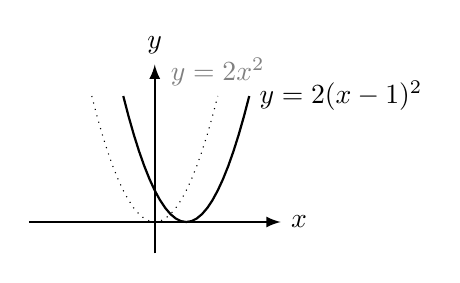
\begin{tikzpicture}[scale=0.4]%倍率
                \draw[thick, -latex] (-4,0)--(4,0) node[right] {$x$};%x軸
                \draw[thick, -latex] (0,-1)--(0,5) node[above] {$y$};%y軸
                \draw[domain=-2:2,dotted] plot(\x, {pow(\x,2)})node[above]{\textcolor{gray}{\(y=2x^2\)}};
                \draw[domain=-1:3,thick] plot(\x, {pow(\x,2)-2*\x+1})node[right]{{\(y=2(x-1)^2\)}};
            \end{tikzpicture}
        \end{center}
        \begin{equation}
            \begin{aligned}
                2(x-1)^2 & = 2(x^2-2x+1) \\
                         & = 2x^2-4x+2
            \end{aligned}
        \end{equation}
    \end{tpscol} &
    \begin{tptcol}
        \begin{framed}
            \noindent\textbf{評価}\\ {\small(主体的に学習に取り組む態度)}\\
            \(x\)軸方向へ平行移動する二次関数のグラフについて関心を持ち,調べようとする.
            \rightline{\fbox{C1}}
        \end{framed}
    \end{tptcol}\vspace{3em}\\
    &&\\
    \hline
    \begin{tpfcol}
        \textbf{振り返り}\\
        二次関数の式とグラフの平行移動について理解する.
    \end{tpfcol} &
    \begin{tpscol}
        \begin{framed}
            \noindent\underline{発展問題}\\
            二次関数\(y=2(x-p)^2\)のグラフは,\(y=2x^2\)のグラフをどのように平行移動したグラフとなるか.
        \end{framed}
    \end{tpscol} & \\
    \begin{tpfcol}
        自己評価をする.
    \end{tpfcol} &
    \begin{tpscol}
        自己評価表を記入する.
    \end{tpscol} &
    \begin{tptcol}
        自己評価表を活用する.
    \end{tptcol} \\
    \hline
\end{TeachingProcedures}
\vspace{2cm}
\hrulefill\\
\verb|http://www.tochigi-edu.ed.jp/icnt/kenshu-c-h29/?action=common_download_main&upload_id=12782 参考|
\end{document}